\section{Introduction}

Construction work entails substantial safety and health risks. The U.S. Bureau of Labor Statistics reported 1,032 fatal occupational injuries in construction and extraction occupations in 2024; common events included falls, slips, trips, and transportation incidents involving construction vehicles or machinery \cite{bls2024}. Beyond traumatic injuries, work with silica-containing materials such as concrete and mortar can expose workers to high concentrations of respirable crystalline silica over long periods, increasing the risks of silicosis, lung cancer, and chronic obstructive pulmonary disease \cite{niosh2024}. Concrete floor leveling and troweling further combine a large work area, repeated passes, and a narrow time window governed by concrete setting. Manual work therefore requires sustained physical exertion and repetitive motion. Field physiological measurements of concrete slab placing and finishing crews showed that most manual workers experienced high energy expenditure and cardiopulmonary demand, with a greater risk of physical fatigue than equipment operators \cite{abdelhamid1999}. Surface finish also depends on operator experience, proficiency, and moment-to-moment condition \cite{albers2004,kobayashi1996}. Releasing workers from hazardous, repetitive, and physically demanding floor operations while improving the consistency of the finished surface is therefore a problem of direct engineering and social value for construction robotics.

Floor-troweling robots provide a practical route toward mechanization. Early field trials showed that a remotely operated troweling robot could perform multiple operations from wood floating to steel troweling. It treated approximately 1,000~m$^2$ across five sites and achieved an average productivity of about 317~m$^2$/h under the reported test conditions \cite{kobayashi1996}. For an order-of-magnitude comparison, the average production rate of manual steel troweling is approximately 13.9~m$^2$/h \cite{methvin2026}; the reported robotic rate is therefore about 22.8 times the rate of one manual worker. Subsequent work introduced electric actuation, laser localization, task planning, and remote monitoring to ride-on power trowels, allowing them to follow specified paths within a predefined floor area \cite{hwangbo1999}.

Most existing troweling robots use a center-mounted or front-mounted disc. Because the tool remains fixed relative to the base, the base path largely determines the tool path, and back-and-forth routes can be planned with a fixed working width \cite{kobayashi1996,hwangbo1999}. Swing-arm configurations have recently attracted attention because they enlarge the end-disc workspace without requiring a large base. Such a robot can place its circular disc beside the base or into locally constrained regions while the base remains clear of walls, columns, and openings, thereby partially decoupling the traversable base path from the tool trajectory. The arm can also increase the effective coverage width. For a fixed-disc platform, the nominal width of a straight pass is mainly limited by the disc diameter. A swing-arm platform can instead move the disc laterally while the base advances, so that the effective width depends on the arm length, angular range, and disc diameter and can exceed the disc diameter \cite{lin2025}. At the same base speed, provided that the swing frequency keeps consecutive sweeps contiguous without introducing gaps, the theoretical covered area per unit time can increase from approximately $v(2R)$ for a fixed disc to $v w_{\mathrm{eff}}$ for a swing arm, where $w_{\mathrm{eff}}>2R$. Previous coverage-planning research likewise shows that repeated coverage, average velocity, and the smoothness of turns jointly affect task time and energy consumption \cite{galceran2013,lee2011}. The swing-arm configuration may also reduce unnecessary driving and sharp turns on wet concrete and provide more admissible poses near corners, narrow-passage entrances, and obstacles \cite{lin2025}.

\begin{figure}[htbp]
  \centering
  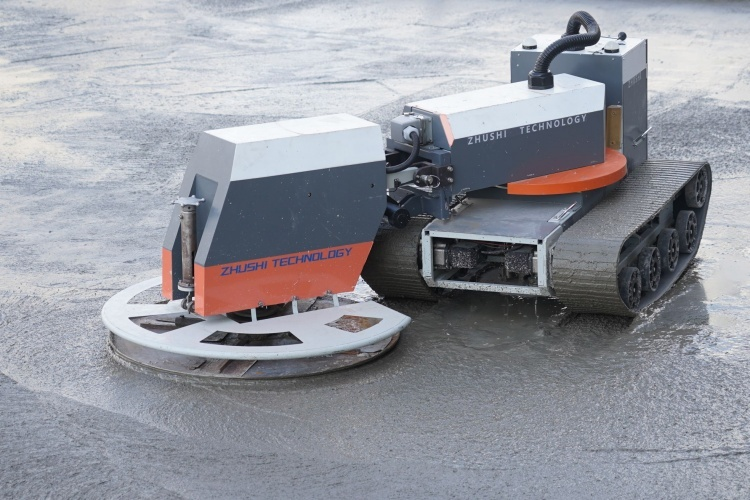
\includegraphics[width=0.82\linewidth]{figure_1_swing_arm_troweling_robot_photo.jpg}
  \caption{A swing-arm troweling robot operating on site. The tracked base, swing arm and actuator, and circular end disc are visible. Image source: Shangguan News; photograph provided by China Construction Eighth Engineering Division.}
  \label{fig:robot-photo}
\end{figure}

Mechanization and teleoperation, however, do not by themselves provide autonomy. A human teleoperator must continuously observe the floor and machine state while coordinating translation, steering, and troweling. In spaces divided by walls, columns, embedded components, and openings, occluded views and fragmented passages increase the burden of global route selection and can cause backtracking, detours, missed regions, and repeated work. Experiments with teleoperated mobile robots also show that manual driving time increases with environmental difficulty and depends on operator skill and the level of obstacle-avoidance assistance \cite{storms2016}. Existing swing-arm systems commonly rely on human--robot cooperation or predefined trajectories and do not yet generate complete coverage routes automatically for complex construction maps \cite{lin2025}. Continuous teleoperation also requires a skilled operator to remain on duty, adding training and on-site supervision costs. Empirical studies of construction-robot adoption further identify economic factors, work culture, and uncertain business returns as barriers to deployment \cite{ocs2024,delgado2019}. Without autonomous coverage planning, these operational burdens remain even after the troweling process is mechanized.

This task is an instance of coverage path planning (CPP): the tool must sweep the target area while avoiding obstacles and controlling missed coverage, repeated coverage, transfer distance, and execution time \cite{galceran2013}. Existing approaches include back-and-forth sweeps after cellular decomposition \cite{choset1998,bahnemann2021}, decomposition and transfers on polygons with holes \cite{polygoncoverage}, grid or spanning-tree traversal \cite{gabriely2001,nobleo}, and strip generation with curvature-constrained connections for fixed-width implements in applications such as agriculture \cite{mier2023,fields2cover}. Mobile-manipulator methods can plan local motions for a base and an end tool \cite{thakar2022}, while SatAOI can identify the workable area of a swing-arm troweling robot in an obstacle map \cite{lin2025}; neither, however, provides a complete continuous coverage route for a complex two-dimensional floor. Section~\ref{sec:related-work} gives a detailed classification and discusses these boundaries.

CPP for a swing-arm troweling robot introduces three interdependent requirements. First, the planner must represent a complex free space containing openings, dense obstacles, and narrow connections. Second, at a fixed base pose, it must distinguish the disc positions and whole-robot collision states associated with different arm angles. Third, while the base moves continuously, actual coverage must be determined from arm angular velocity and the continuous disc sweep rather than from a static reachability envelope. A static reachability envelope is the region the arm can touch in some poses and does not include the time course of base travel and swing-arm motion. Simply dilating the base path into a constant-width strip cannot satisfy all three requirements. Consequently, prior work lacks a complete planning chain from a construction map through decomposition and visitation order to coordinated base--arm motion and end-tool coverage evaluation.

This paper proposes BiRect, a hierarchical coverage path planning method that places bidirectional rectangular decomposition, the visitation order on a feasible transition graph, and the coverage ratio and execution time computed from the area actually swept by the circular disc in one chain, using the same base--swing-arm--disc model for the map, local motion, and trajectory evaluation.

The remainder of the paper is organized as follows. Section~\ref{sec:related-work} reviews the development of concrete-troweling robots and the challenges posed by obstacle-rich construction environments, compares representative CPP methods, and summarizes the unresolved research gap. Section~\ref{sec:methodology} presents the robot and environment models, rectangular-candidate decomposition, connectivity completion, global visitation, and swing-assisted coverage within each rectangle. Section~\ref{sec:experiments} evaluates the method through a baseline comparison, candidate-scan strategy experiments, and a speed-sensitivity study. Section~\ref{sec:conclusion} summarizes the experimentally supported contributions, limitations, and future work.

\section{Related Work}
\label{sec:related-work}

\subsection{Concrete Troweling Robots and Application Challenges}

After concrete has been placed and initially leveled, it must be troweled repeatedly before setting and hardening. Troweling removes local height variations and rough texture, redistributes the surface paste, and produces a flat, dense finish through compaction and polishing. The operation covers a large area and is highly repetitive, while its start time, speed, and number of passes are constrained by the state of concrete setting. Starting too early can disturb an unstable surface; starting too late can prevent the desired flatness and finish. Site practice has therefore long depended on the experience and continuous involvement of skilled workers \cite{albers2004,kobayashi1996}. A troweling robot moves the disc and treats the surface at a relatively stable speed and cadence, reducing physical workload and the effect of worker-state variability on quality consistency \cite{kobayashi1996,shin2003}. Its role is thus not merely to replace a hand tool, but to convert a process that requires continuous manual operation into one that a mechanical system can execute consistently.

The evolution of concrete-troweling equipment can be understood along two axes: the disc--base relationship and the mode of control.

Along the disc--base relationship, existing troweling robots fall into three configurations. A center-mounted disc lies under or near the center of the base, as on the ride-on twin-rotor machine \cite{hwangbo1999} and on the twin-disc machine whose discs sit under the body and whose travel follows disc attitude \cite{shin2003}. A front-mounted arrangement places troweling discs at both the front and the rear of the travel mechanism; the discs stay fixed relative to the base and have no active lateral motion \cite{kobayashi1996}. A swing-arm configuration places the disc at the end of an actively rotating arm \cite{lin2025}. The swing arm can send the disc into regions beside walls, columns, openings, and narrow passages while the base stays clear of them. When consecutive sweeps remain contiguous, the same base speed can give an effective coverage width larger than the disc diameter. This configuration has received increasing attention in recent construction-robot research \cite{lin2025}. These advantages come from coordinating base translation with swing-arm motion and cannot be represented by a fixed-width strip model.

\begin{figure}[htbp]
  \centering
  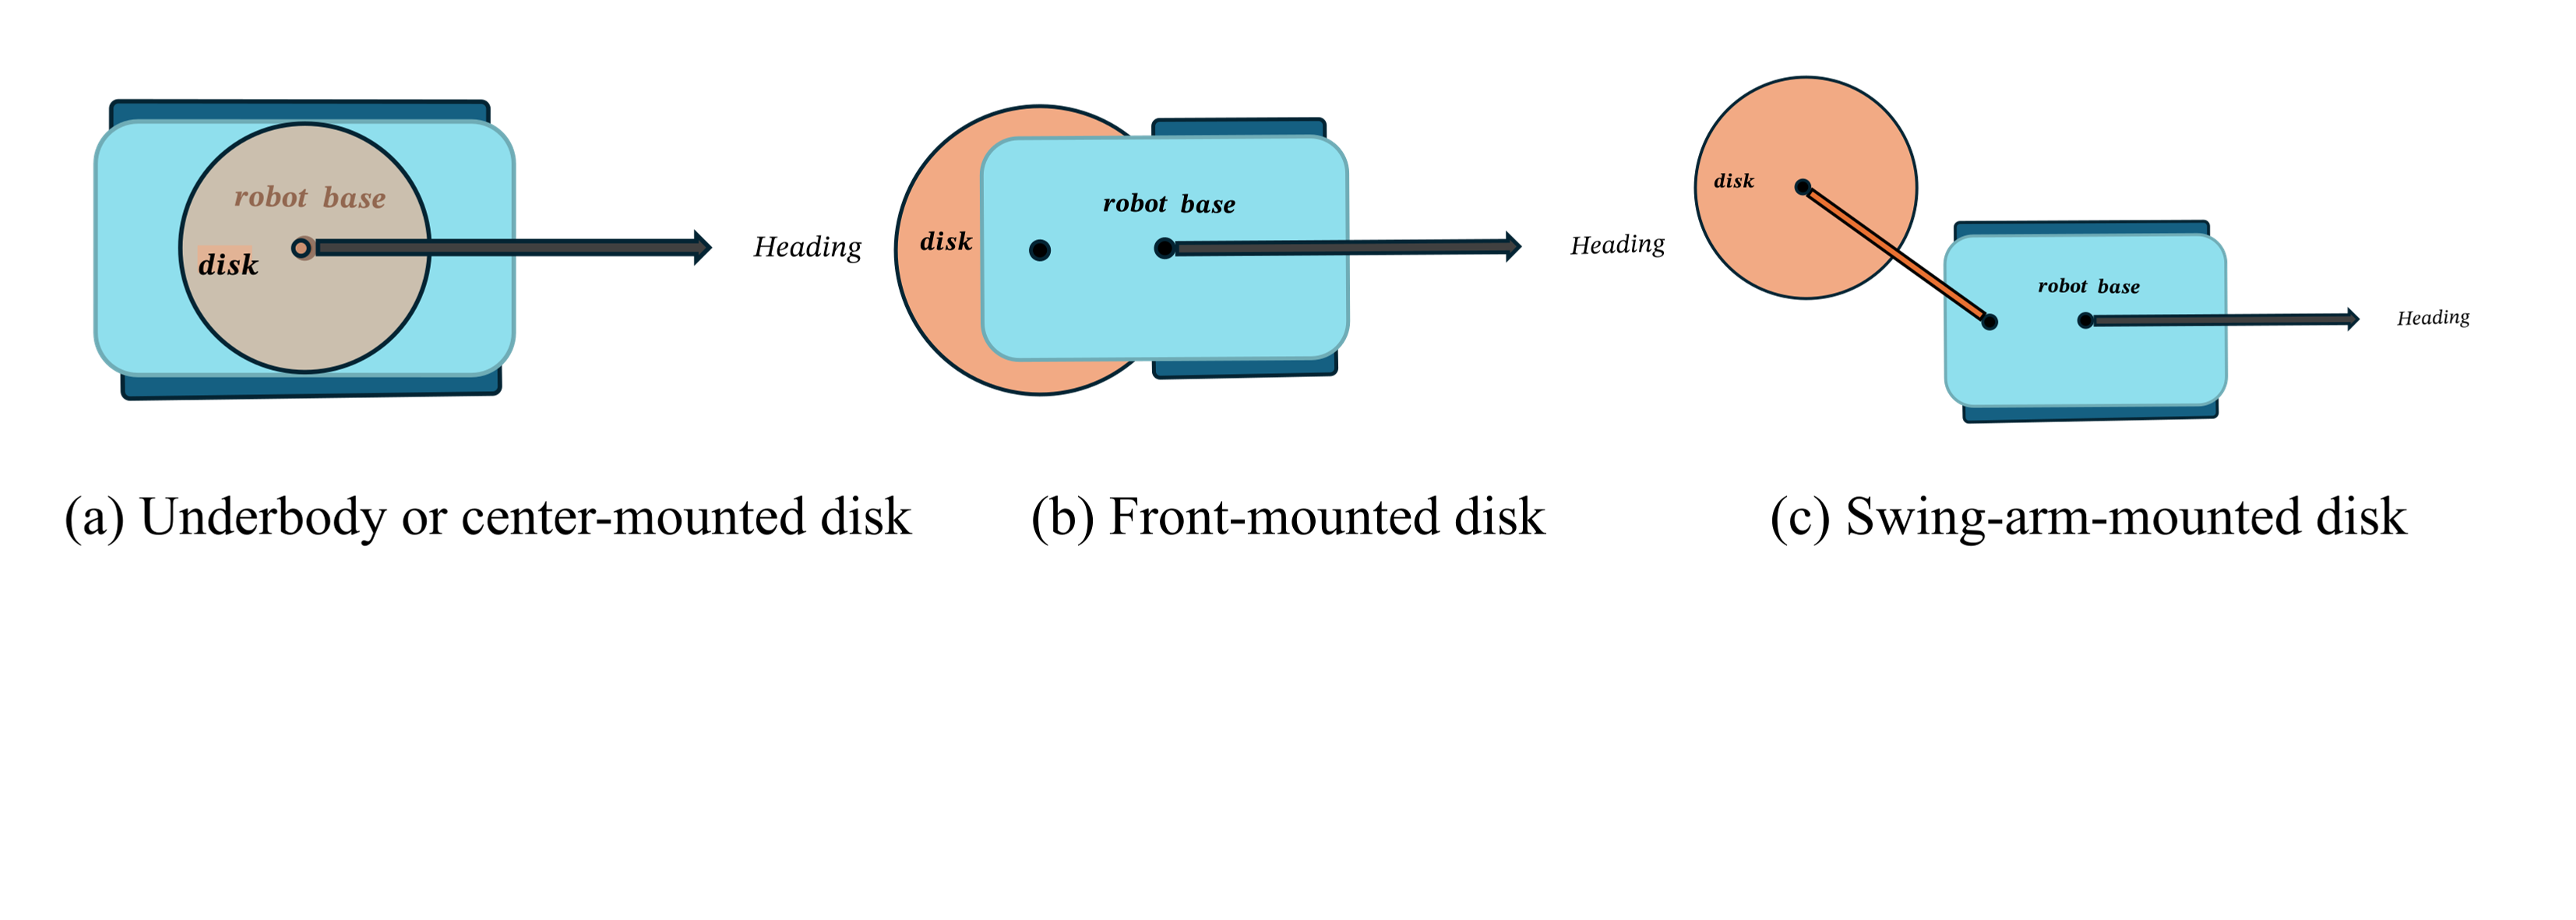
\includegraphics[width=0.92\linewidth]{figure_2_disc_vehicle_relationships.png}
  \caption{Three arrangements of the troweling disc relative to the base: (a) center-mounted; (b) front-mounted; and (c) swing-arm. Arrows indicate the direction of base travel.}
  \label{fig:disc-configurations}
\end{figure}

The state variables $x_c$ and $y_c$ locate the center of the base in the ground frame, $\theta$ is the base heading, and $\phi$ is the arm angle relative to the base. Together, the four variables determine the poses of the base, swing arm, and disc in the construction plane. A region traversable by the base is not necessarily reachable by the disc, and a disc-reachable pose is not necessarily collision-free for the complete mechanism. Planning must therefore check the geometry of all three components and coordinate the base and swing arm throughout continuous motion \cite{lin2025}.

Along the mode of control, the equipment falls into three modes: manual walk-with or ride-on, wireless teleoperation, and autonomous travel in regular areas. Walk-behind and ride-on power trowels first mechanized the operation, but a worker still walked with or rode on the machine. Because the disc remained fixed relative to the base, the machine route effectively determined the disc trajectory \cite{hwangbo1999}. Wireless teleoperation then moved the operator outside the work area. Kobayashi et al.\ fixed front and rear troweling discs to a lightweight mobile base and used wireless teleoperation and taught-motion replay to perform successive operations from wood floating to steel troweling \cite{kobayashi1996}. The system reduced worker exertion, but the discs still moved rigidly with the base, and coverage remained sensitive to operator experience, floor friction, and steering behavior \cite{kobayashi1996}. Autonomous travel in regular areas came next. Hwangbo et al.\ retained the fixed twin-rotor troweling mechanism of a ride-on machine, electrified controls such as steering, blade pitch, and acceleration, and added laser localization, reflective landmarks, and a construction-drawing-based task planner. The resulting machine could work autonomously along a prescribed pattern or planned route \cite{hwangbo1999}. This improved control autonomy without changing the rigid coupling between disc and body.

A swing arm makes the disc movable relative to the base, so autonomous travel with a fixed disc is not enough for the platform studied by SatAOI. SatAOI starts from an obstacle grid, models the base, swing arm, and disc, and searches for connected regions that the robot can enter and in which the disc can operate \cite{lin2025}. Its output stops at that workable area: it gives no visitation order, no base transfer between regions, and no coordinated base--swing-arm coverage inside a region. This paper starts from that area and plans a continuous coverage route.

\subsection{Coverage Path Planning Methods}

Existing CPP methods can be compared along two dimensions: map-representation capability and fidelity of robot-behavior modeling. The first describes whether a planner can represent irregular boundaries, multiple obstacles, holes, and narrow connections and use them to establish adjacency and feasible transfers between coverage regions. The second describes whether the planner captures the physical dimensions, relative poses, motion modes, and collision constraints of the robot and tool rather than replacing the operation with a point, disc, or fixed-width strip. These dimensions define four capability classes, and the names below are those used in this paper. Idealized coverage methods are weak in both map representation and robot-behavior fidelity, and they mainly establish fundamental coverage mechanisms. Map-enhanced methods represent a complex map but keep a fixed tool footprint. Platform-constrained methods describe motion constraints in detail but primarily target regular or local workspaces. Environment--platform coupled methods retain both a complex map and realistic robot behavior.

\begin{figure}[htbp]
  \centering
  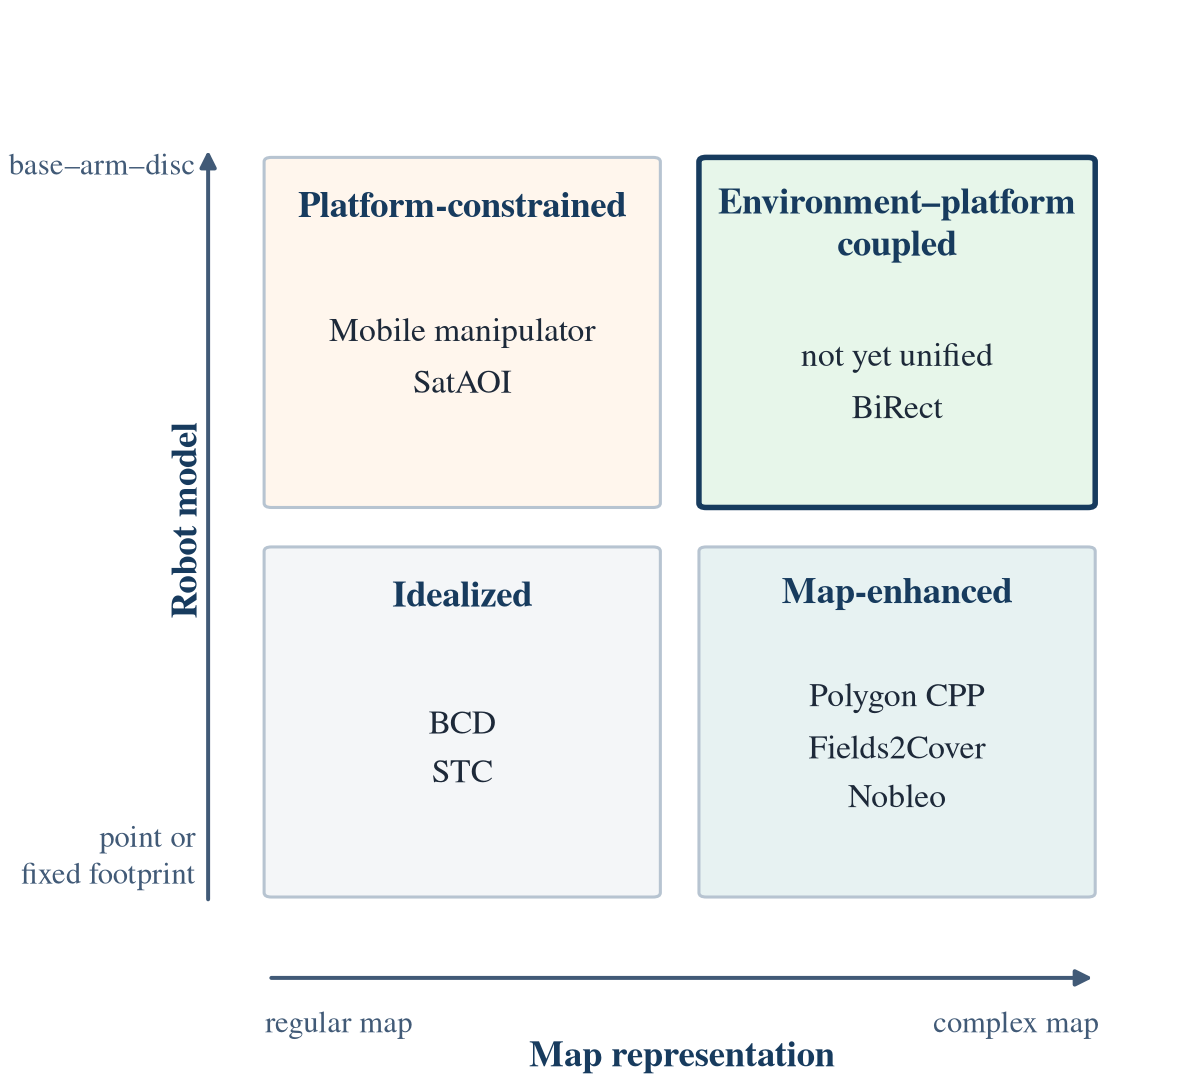
\includegraphics[width=0.88\linewidth]{figure_cpp_class_quadrant.png}
  \caption{Four capability classes arranged by map representation and robot model.}
  \label{fig:cpp-classes}
\end{figure}

The first class comprises classical coverage algorithms that express the core coverage idea clearly but generally close the problem only for idealized maps and simplified robot models. Representative methods include Boustrophedon Cellular Decomposition (BCD) and Spanning Tree Coverage (STC). BCD scans the free space and ends the current cell when the number of free intervals on the scan line changes, then generates back-and-forth sweeps inside the cell \cite{choset1998}. STC coarsens the free space into a grid, builds a spanning tree on that grid, and walks the fine cells around the tree boundary \cite{gabriely2001}. These methods establish the respective roles of cellular decomposition and graph traversal. They do not represent the relative position of the base and the disc, nor the change of the arm angle $\phi$, and are therefore difficult to apply to swing-arm troweling, on which the disc moves relative to the base.

The second class can represent complex maps, but the robot and tool are still modeled mainly by a fixed footprint. It first represents a map with holes, non-convex boundaries, or obstacles, then covers that map with fixed-width strips, orders the regions, and connects them by collision-free turns. Reproducible examples include ETH Zurich's \texttt{polygon\_coverage\_planning} \cite{bahnemann2021,polygoncoverage}, Fields2Cover for agricultural vehicles \cite{mier2023,fields2cover}, and the Nobleo Full Coverage Path Planner for ROS occupancy grids \cite{nobleo}. \texttt{polygon\_coverage\_planning} handles general polygons with holes, uses BCD or trapezoidal decomposition to generate cells, constructs multiple sweep candidates for each cell, and performs global selection and collision-free transfer through an Equality Generalized Traveling Salesman Problem and a visibility graph. Fields2Cover supports non-convex fields, obstacles, headlands, swaths, and route ordering, and connects swaths by curvature-constrained Dubins or Reeds--Shepp connections \cite{mier2023,fields2cover}. Nobleo's planner implements a Backtracking Spiral Algorithm/Spiral-STC-type method \cite{nobleo} on a ROS occupancy grid and permits separate robot and tool radii. These frameworks show that complex boundaries, obstacles, and engineering interfaces can be addressed systematically. Their tool width, implement width, or tool disc nevertheless remains essentially fixed relative to the base and cannot represent the time-varying sweep caused by continuous changes in $\phi$.

The third class retains, during planning, the minimum turning radius, the reachable range of the arm, and component collisions, while its scenes are mostly regular sites, local surfaces, or three-dimensional objects. It includes the nonholonomic vehicle connections in Fields2Cover and mobile-manipulator surface-coverage methods for tasks such as spray disinfection. Fields2Cover incorporates minimum turning radius and vehicle kinematics \cite{mier2023,fields2cover}, but targets agricultural swaths with a fixed implement width. Mobile-manipulator studies explicitly handle the base, arm, end tool, reachability, and occlusion. For example, spray-based surface disinfection can generate end-effector paths from three-dimensional surfaces and jointly select base positions and arm motions \cite{thakar2022}. Such methods describe how a robot executes a task in greater detail, but generally target regular sites, agricultural strips, or three-dimensional object surfaces rather than jointly performing obstacle handling, area decomposition, global traversal, and continuous ground-coverage evaluation on a known two-dimensional construction map.

Swing-arm troweling therefore requires the fourth class shown in Fig.~\ref{fig:cpp-classes}. Walls, columns, reserved openings, and narrow corridors divide the floor into irregular regions with complex connectivity, which the planner must represent and visit continuously. Meanwhile, the disc position is jointly determined by base motion and active swing-arm motion; coverage and collision status vary continuously with base heading and arm angle and cannot be approximated by a fixed footprint. A complete, continuous, and executable route therefore requires the construction map and the coordinated base--swing-arm--disc behavior to be represented in the same planning model.

Research has thus advanced in both complex-map representation and robot-behavior modeling, but the two have not yet been unified, especially for swing-arm floor coverage. CPP frameworks with strong map support usually assume a fixed tool footprint and cannot describe the dynamic coverage created by a rotating arm. Methods that model vehicle kinematics, manipulator reachability, and component collisions in detail generally focus on regular sites, local operations, or three-dimensional surfaces and do not fully decompose and continuously traverse a complex two-dimensional construction map. SatAOI considers both an obstacle map and the geometry of the base, arm, and disc, but stops at delimiting the workable area and does not produce a visitation order, transfer route, or coordinated coverage trajectory within each region \cite{lin2025}. The central gap is therefore a swing-arm troweling CPP method that combines complex-map processing with high-fidelity robot-behavior modeling and generates a complete, continuous, executable route directly from the construction map.

Table~\ref{tab:cpp-comparison} compares representative approaches along these two dimensions. Work spanning more than one class is placed according to its principal contribution: Fields2Cover is treated as map-enhanced and SatAOI as platform-constrained. The stated limitations concern direct application to a mobile base with an active arm and circular disc; they are not general judgments of the methods or software.

\begin{longtable}{@{}>{\raggedright\arraybackslash}p{0.13\linewidth}>{\raggedright\arraybackslash}p{0.15\linewidth}>{\raggedright\arraybackslash}p{0.14\linewidth}>{\raggedright\arraybackslash}p{0.16\linewidth}>{\raggedright\arraybackslash}p{0.30\linewidth}@{}}
\caption{Representative CPP methods and their applicability to swing-arm troweling.}\label{tab:cpp-comparison}\\
\toprule
Category & Representative method & Map representation & Robot model & Pros and cons \\
\midrule
\endfirsthead
\toprule
Category & Representative method & Map representation & Robot model & Pros and cons \\
\midrule
\endhead
Idealized coverage & BCD \cite{choset1998} & Cellular decomposition & Fixed footprint & $\checkmark$ Organizes back-and-forth sweeps within cells.\newline $\times$ Does not represent an active arm or continuous sweep. \\
Idealized coverage & STC \cite{gabriely2001} & Grid spanning tree & Point or disc robot & $\checkmark$ Systematically traverses a grid.\newline $\times$ Cannot use the time-varying disc position created by arm motion. \\
Map-enhanced & Polygon CPP \cite{bahnemann2021,polygoncoverage} & Polygon with holes & Fixed footprint & $\checkmark$ Provides alternative strips and obstacle-avoiding transfers.\newline $\times$ Does not represent the arm's instantaneous disc position. \\
Map-enhanced & Fields2Cover \cite{mier2023,fields2cover} & Non-convex field & Fixed footprint & $\checkmark$ Includes swaths, route ordering, and curvature-constrained connections.\newline $\times$ The fixed footprint omits arm motion. \\
Map-enhanced & Nobleo FCPP \cite{nobleo} & Occupancy grid & Fixed footprint & $\checkmark$ Integrates grid coverage with a navigation stack.\newline $\times$ Does not coordinate arm angle, arm angular velocity, and base speed. \\
Platform-constrained & Mobile-manipulator surface coverage \cite{thakar2022} & Three-dimensional surface & Mobile manipulator & $\checkmark$ Jointly plans base placement and end-tool motion.\newline $\times$ Does not completely traverse a complex two-dimensional floor. \\
Platform-constrained & SatAOI \cite{lin2025} & Construction obstacle map & Base, arm, and disc & $\checkmark$ Determines workable regions and connectivity.\newline $\times$ Does not generate a visitation order or continuous coverage trajectory. \\
Proposed method & BiRect & Two-dimensional obstacle map & Swing arm with a time-varying disc & $\checkmark$ Links rectangular decomposition, visitation, local swinging, and trajectory evaluation.\newline $\times$ Currently assumes a static map and uses heuristic search. \\
\bottomrule
\end{longtable}

\subsection{Summary and Research Gap}

Prior work provides several capabilities needed here, but has not solved complex-map coverage within one unified task. BCD \cite{choset1998} and STC \cite{gabriely2001} can represent two-dimensional free spaces and can decompose regions or traverse grids. Decomposition and swath generation on regions with holes or non-convex boundaries are given in \cite{bahnemann2021,polygoncoverage}, and grid traversal in \cite{nobleo}. With a tool fixed to the base, they can arrange adjacent sweeps according to a prescribed width. Fields2Cover additionally generates turns and curvature-constrained connections for vehicles whose direction and minimum turning radius prevent arbitrary lateral motion \cite{mier2023,fields2cover}. Mobile-manipulator research addresses end-tool reachability and collision relationships \cite{thakar2022}, while SatAOI uses the geometry among the base, swing arm, disc, and obstacles to delimit regions the robot can enter and the disc can treat \cite{lin2025}. These abilities remain distributed across different task models and applications: complex-map CPP usually assumes a fixed footprint, detailed robot models are commonly used for local or regular workspaces, and SatAOI terminates at workable-area delimitation. For the specific objective of generating a complete executable route for a swing-arm troweling robot in a known, complex, two-dimensional construction map, three coupled gaps remain.

First, existing CPP methods do not model active swing-arm behavior sufficiently to plan the actual coverage of the disc: in conventional CPP the tool is fixed to the base, so determining the base route also determines coverage. At the same base position and heading, a different arm angle places the disc center on an arc whose radius is the arm length, and the whole-robot collision state differs as well. Maximum arm reach, or a widened strip, only shows that some pose can reach a location; it is not coverage during continuous motion.

Second, complex-map decomposition and local swing motion have not been integrated into a computationally practical planning chain. SatAOI stops at the workable area; this paper uses a hierarchical heuristic to join region connectivity, visitation order, and coordinated base--swing-arm coverage inside each region into one computable chain.

Third, a static reachability envelope does not guarantee complete coverage during dynamic execution, and prior work does not explicitly model base--arm velocity coupling, the coordination of base linear velocity and arm angular velocity. Maximum arm reach indicates only which locations the disc can touch in some poses. While the base advances continuously and the swing arm swings periodically, the longitudinal spacing between consecutive sweeps is determined by base speed and arm angular velocity; if the base is too fast or the swing arm too slow, untreated gaps remain even when the target lies inside the static reachability envelope defined above, so being reachable is not the same as being covered.
